\section{Troubleshooting}

\begin{frame}
\frametitle{Describe}
É possível ver mais informações sobre determinado recurso ou grupo de recursos
\begin{figure}[htpb]
	\centering
	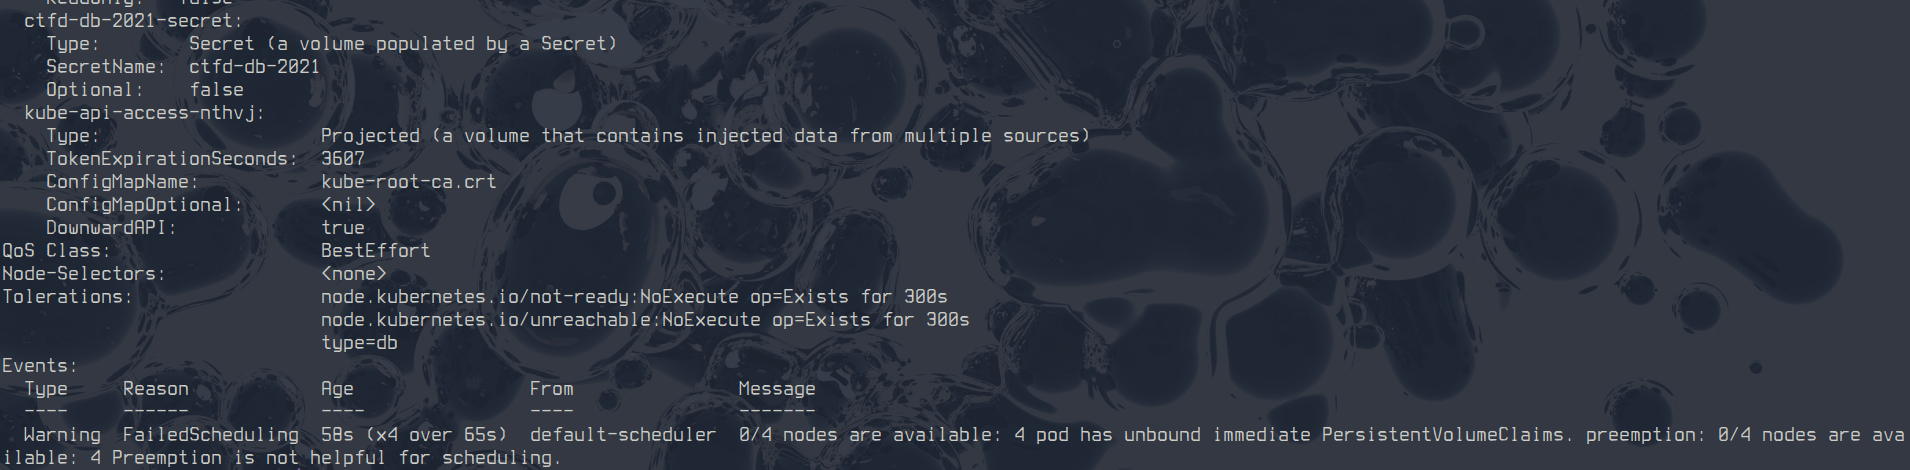
\includegraphics[width=\textwidth]{Kubectl_describe}
	\caption{Motivo de falha do banco de dados}
\end{figure}
\end{frame}

\begin{frame}
\frametitle{Logs}
Possibilita ver a causa de erro dentro do container:
\begin{figure}[htpb]
	\centering
	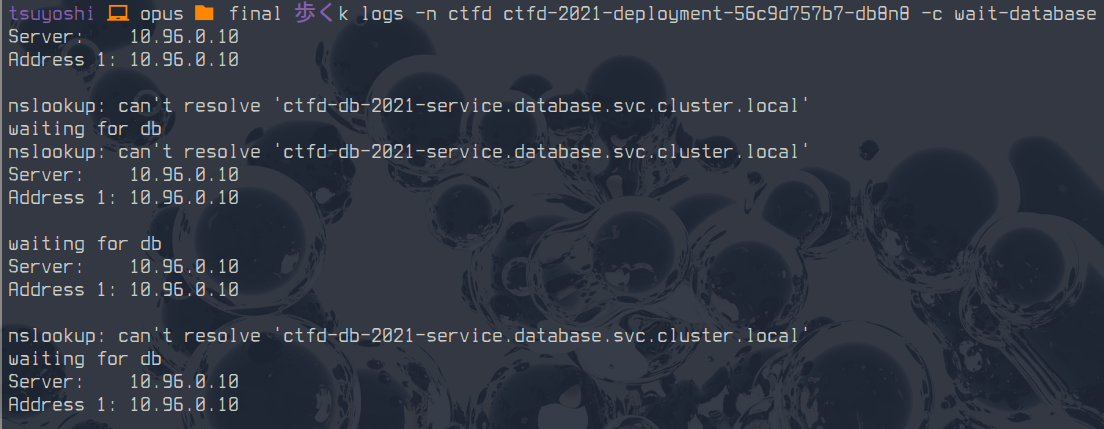
\includegraphics[width=\textwidth]{Kubectl_logs}
	\caption{Log do \textit{initContiner}}
\end{figure}
\end{frame}

\begin{frame}
\frametitle{exec}
Verificar \textit{Mounts, secrets, env, conexão, etc\dots}:
\begin{figure}[htpb]
	\centering
	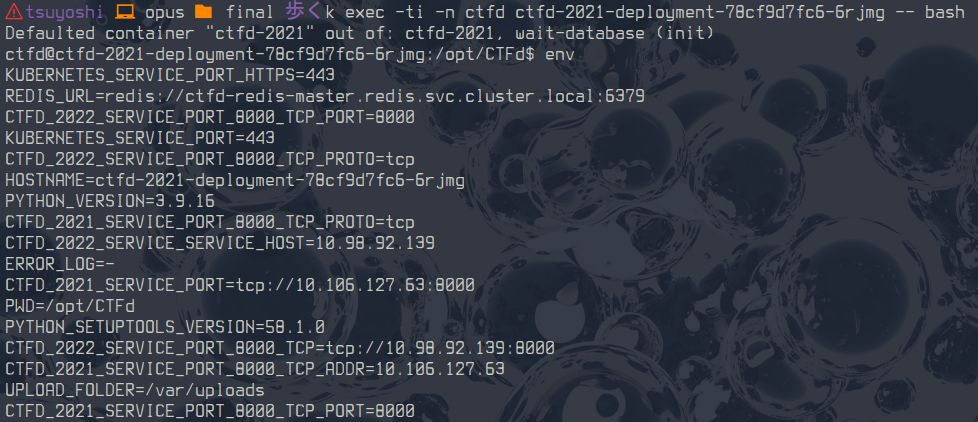
\includegraphics[width=\textwidth]{Kubectl_exec}
	\caption{Verificar variáveis de ambiente}
\end{figure}
\end{frame}

\begin{frame}
\frametitle{events}
\begin{itemize}
	\item Os eventos são um relatório de um evento que ocorreu dentro do \textit{cluster}
	\item \uncover<2->{Os eventos são informativos e infomações adicionais}
\end{itemize}

\uncover<3->{
\begin{figure}[htpb]
	\centering
	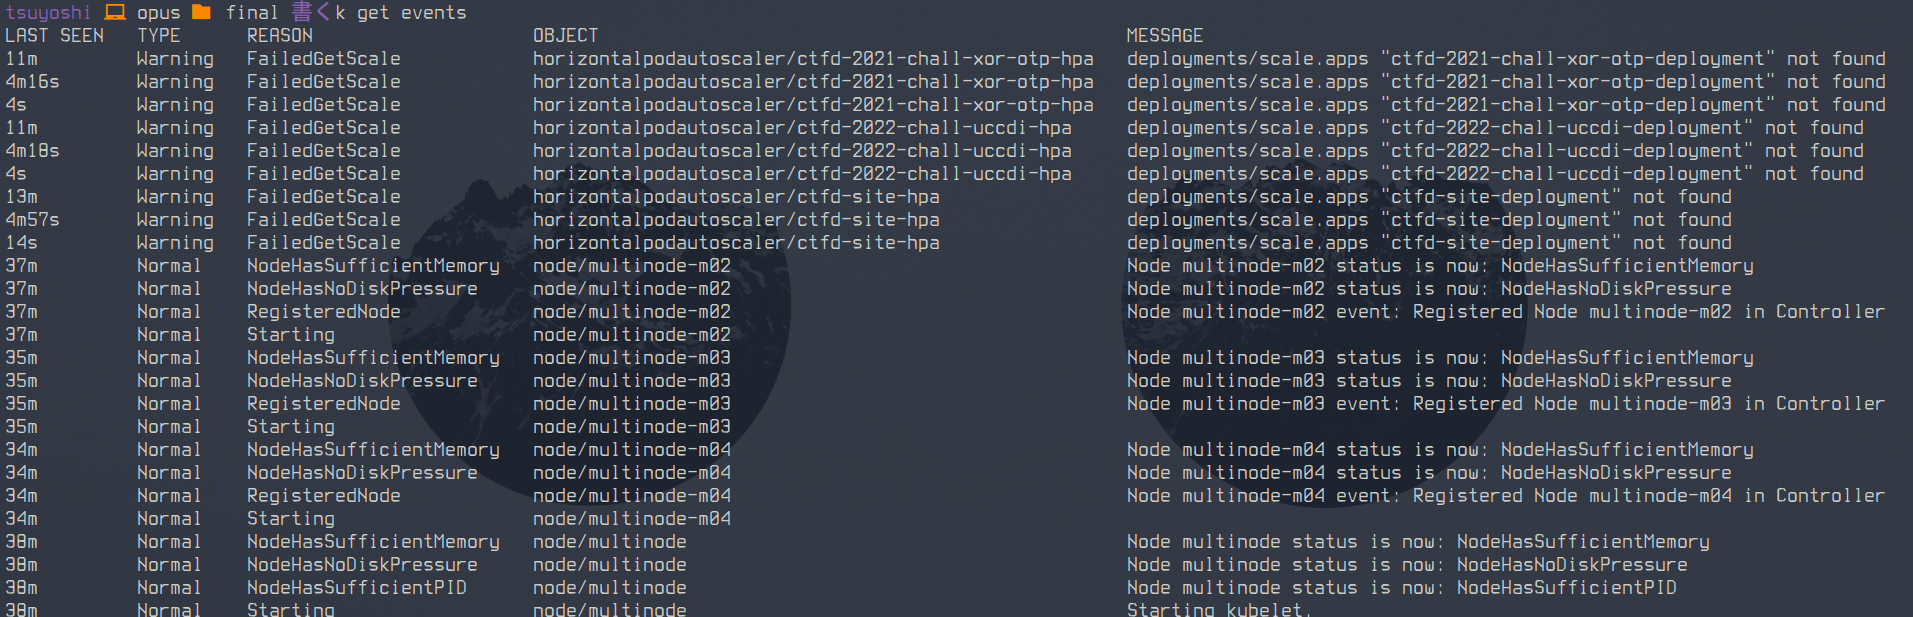
\includegraphics[width=\textwidth]{Kubectl_events}
	\caption{Eventos}
\end{figure}
}
\end{frame}
